% ----------------------------------------------------------
\chapter{Fundamentação Teórica}
% ----------------------------------------------------------
Neste capítulo são mostrados os fundamentos necessários para entender os conceitos abordados no presente trabalho.


\section[Treinamento de barra fixa para o TAF]{Treinamento de barra fixa para o TAF}\label{sec:Treinamento de barra fixa para o TAF}

\subsection[Teste de Aptidão Física]{Teste de Aptidão Física}\label{sec:Teste de Aptidão Física}

O \ac{TAF}  é uma etapa comum em concursos públicos para provimento de cargos em carreiras relacionadas a área de segurança pública, seu objetivo é atestar a capacidade do indivíduo em desempenhar funções específicas do cargo por meio da avaliação de determinados exercícios. A avaliação é embasada em exercícios e parâmetros preestabelecidos em edital como por exemplo: quantidade de repetições de um determinado movimento para o exercício de barra fixa ou flexão abdominal, tempo gasto para translocação em uma determinada distancia nas corridas de 12km, 2.400m ou natação, ou até mesmo a distância percorrida durante o salto de impulsão horizontal\cite{TAF_adv}.


\subsection[Barra Fixa]{Barra Fixa}\label{sec:Barra Fixa}

O teste de flexão em barra fixa, ou teste dnâmico de barra fixa, apresenta variações de acordo com os seguintes editais: Concurso público para admissão ao curso de formação de soldados Bombeiros Militar do quadro de praças (QP-BM) e do quadro de praças especialistas (QPE-BM) do Corpo de Bombeiros Militar de Minas Gerais para o ano de 2020 \cite{eCBMG2018}; Concurso público para admissão ao curso de formação de soldados do quadro de praças especialistas da Polícia Militar de Minas Gerais \cite{ePMMG2021}; Concurso público para o provimento de vagas nos cargos de delegado de Polícia Federal, agente de Polícia Federal, escrivão de Polícia Federal e papiloscopista Policial Federal \cite{ePF2021}; Concurso público para o provimento de cargos da carreira de agente de segurança penitenciário/policial penal do quadro de pessoal da Secretaria de Estado de Justiça e Segurança \cite{ePP2021}.

No entanto, os princípios do movimento permanecem semelhantes:

\begin{itemize}

    \item A barra fixa é instalada a uma altura tal, que o avaliado, mantendo-se pendurado, com os cotovelos em extensão, não tenha contato dos pés com o solo;

    \item A posição da pegada é pronada (dorso da mão voltado para o rosto) e a abertura das mãos corresponde à distância biacromial (largura dos ombros);

    \item Após assumir essa posição, o avaliado deverá elevar o corpo até que o queixo ultrapasse o nível da barra, após o que retornará à posição inicial;

    \item O movimento é repetido tantas vezes quanto possível, sem limite de tempo.

    \item Os cotovelos deverão estar em extensão total para o início de flexão;

    \item É permitido repouso entre um movimento e outro, contudo, o avaliado não poderá tocar os pés no solo;

    \item Não são permitidos movimentos de quadris ou pernas e extensão da coluna cervical como formas de auxiliar na execução da prova.

    \item A não extensão total dos cotovelos antes do início de nova execução é considerado um movimento incorreto, o qual não será computado no desempenho do candidato.

    \item Somente é contado o número de movimentos completados corretamente.

\end{itemize}

\begin{figure}[!htb]
	\centering
    \caption{Movimento de barra fixa}
	\includegraphics[scale=0.7]{figuras/TAF/barraFixa.jpg}
    \legend{Fonte:\cite{barraFixa_IMG}.}
	\label{fig:Movimento de barra fixa}
\end{figure}


\subsection[Feedback]{Feedback}

Feedback é um processo de comunicação que envolve a transmissão de informações sobre o desempenho ou comportamento de uma pessoa ou grupo, com o objetivo de fornecer orientação e incentivo para a melhoria contínua. 

No contexto do treinamento físico, o feedback pode ser fornecido por um treinador ou por uma ferramenta tecnológica, como um aplicativo de treino ou um dispositivo de monitoramento de desempenho. Esse tipo de feedback permite que o indivíduo ajuste sua técnica ou intensidade do exercício durante a atividade, melhorando assim o resultado final \cite{feedback}.




\subsection[Planos anatômicos e eixo de movimento]{Planos anatômicos e eixo de movimento}

Os planos cardinais, também chamados de planos anatômicos, são três planos imaginários que dividem o corpo humano em seções para estudo e referência anatômica. São eles: o plano sagital, que divide o corpo em metades esquerda e direita; o plano frontal (ou coronal), que divide o corpo em partes anterior (frente) e posterior (costas); e o plano transversal (ou axial), que divide o corpo em partes superior e inferior \cite{cinesiologia}.

Cada plano tem um eixo perpendicular utilizado para caracterizar os movimentos referêntes a esse plano. O eixo sagital ou medial-lateral é responsável pelos movimentos de flexão e extensão, o eixo frontal ou anterior-posterior é responsável pelos movimentos de abdução e adução, e o eixo transversal, também conhecido como eixo látero-lateral, é responsável pelos movimentos de rotação medial e lateral\cite{cinesiologia}.


\begin{figure}[!htb]
	\centering
    \caption{Planos anatômicos}
	\includegraphics[scale=0.15]{figuras/TAF/planos.png}
    \legend{Fonte:\cite{planosAnatomicos_IMG}.}
	\label{fig:Planos anatomicos}
\end{figure}


\subsection[Articulação]{Articulação}
A articulação é a conexão de duas ou mais superfícies ósseas que promovem movimento \cite{articulacao}


\subsection[Flexão e Extensão]{Flexão e Extensão}
Anatomicamente, o movimento de flexão refere-se à redução do ângulo entre dois ossos ou partes do corpo no plano sagital ao redor do eixo transverso, o que resulta em um movimento que diminui a distância entre as duas estruturas. Em contraste, a extensão envolve aumentar o respectivo ângulo. \cite{flexao}.


\subsection[Inserção e Origem Muscular]{Inserção e Origem Muscular}
Inserção é a extremidade do músculo que está fixada a um ponto móvel ou a uma peça óssea que se desloca. Em contraste, a origem é a extremidade do músculo que está fixada a um ponto fixo ou a uma peça óssea que não se desloca \cite{sisMuscular}.


\subsection[Parte Distal]{Parte Distal}
A parte distal é o ponto mais afastado do tronco ou do ponto de origem \cite{distal}.



\subsection[Cadeia Cinemática]{Cadeia Cinemática}
Os termos cadeia cinemática aberta ou fechada, são usados para demonstrar se o segmento mais distal da cadeia está fixado a algum objeto imóvel ou até mesmo o solo.

Sendo que cadeia cinemática aberta representa uma situação em que a extremidade do membro não está fixada ao solo ou a algum objeto imóvel e assim, o segmento está livre para se mover e cadeia cinemática fechada representa uma situação em que o segmento mais distal da cadeia está fixo ao solo ou a um objeto imóvel \cite{silva2015cinesiologia}.


\subsection[Ativação Muscular]{Ativação Muscular: Concêntrica, Excêntrica e Isométrica}

Existem diversas formas de ativação muscular, cada uma com características próprias. Uma delas é a ativação isométrica, na qual um músculo produz força sem que haja uma mudança aparente no ângulo articular. Também conhecida como contração estática ou sustentação, a ativação isométrica é importante para estabilizar as articulações durante atividades funcionais, ajudando a prevenir lesões \cite{cinesiologia}.

A ativação concêntrica é outra forma de ativação muscular em que o músculo produz força encurtando-se, ou seja, os pontos de inserção proximal e distal do músculo se aproximam, o que resulta em movimento visível na direção da força. Essa atividade concêntrica produz aceleração dos segmentos do corpo \cite{cinesiologia}.

Por fim, a ativação excêntrica ocorre quando o músculo produz força alongando-se, distanciando seus pontos de inserção proximal e distal e resultando em movimento visível, mas em direção oposta à da força produzida pelo músculo. Essa atividade excêntrica desacelera os segmentos corporais e oferece amortecimento \cite{cinesiologia}.

Portanto o movimento concêntrico é também conhecido como trabalho positivo, em que o músculo exerce força para produzir movimento de uma articulação. Já o movimento excêntrico é chamado de trabalho negativo, ocorrendo quando uma força externa produz o movimento articular enquanto o músculo controla seu nível de ocorrência.



\subsection[Velocidade de Contração]{Velocidade de contração}
De acordo com Bunnstrom (\citeyear{cinesiologia}) velocidade é uma medida da taxa de deslocamento em uma direção específica, é importante destacar que a velocidade de encurtamento ou alongamento do músculo é um fator crítico que afeta a força que pode ser desenvolvida durante a ativação muscular.

Conforme a velocidade da contração concêntrica se torna mais lenta, o desenvolvimento da força muscular aumenta pois a capacidade de produzir força no movimento concentrico está relacionada ao número de conexões entre filamentos de actina e miosina que podem ser formadas por unidade de tempo.

Por outro lado, quando o músculo se alonga durante a atividade, a relação entre velocidade de contração e produção de força é diferente da que ocorre com o encurtamento muscular, pois a força muscular aumenta com o aumento da velocidade durante a contração excêntrica até que a velocidade atinja um ponto no qual o músculo é incapaz de controlar a sobrecarga.






%\subsection[Biceps Braquial]{Biceps Braquial}
%De acordo com Kapandji (\citeyear{movimentoCotovelo}) o bíceps braquial é o principal músculo responsável pela flexão do cotovelo, juntamente com outros dois músculos, o braquial anterior e o braquiorradial.

%A inserção inferior do músculo em questão está localizada na tuberosidade bicipital do rádio. Já as suas inserções superiores, por se tratar de um músculo biarticular, que se encontra na escápula, sendo compostas por duas porções distintas: a primeira, chamada de porção longa, localiza-se no tubérculo supraglenoide após atravessar a articulação ; e a segunda, denominada de porção curta, situada no bico do processo coracoide. 

%A sua ação secundária, porém importante, é a supinação, máxima quando o cotovelo está fiexionado a 90°.



%\subsection[Insuficiência Passiva]{Insuficiência Passiva}

%Quando os músculos se alongam sobre duas ou mais articulações simultaneamente, eles podem chegar ao estado de insuficiência passiva onde é incapaz de alogar e manter a tensão adequada para produzir força. ou seja ocorre a diminuição da capacidade de produção de força. \cite{cinesiologia}

%\subsection[Insuficiência Ativa]{Insuficiência Ativa}

%A insuficiência ativa ocorre em músculos multiarticulares quando estes se encontram no seu comprimento mais curto. Nesse estado, as fibras musculares estão sobrepostas em um grau máximo, o que limita a capacidade do músculo de produzir força ativa, pois de acordo com relação comprimento-tensão de um músculo, a força máxima de um musculo ocorre quando ele está em seu comprimento de repouso e quanto mais ele se encurta mais ele se torna fraco devido a incapacidade de gerar mais contração muscular devido a dificudlade em gerar pontes cruzadas de actina e miosina.\cite{cinesiologia}



\section[Visão computacional]{Visão computacional}
Visão computacional é a ciência que estuda e desenvolve tecnologias que permitem extrair características de imagens capturadas por diferentes tipos de sensores e então permitem reconhecer, manipular e processar dados sobre os objetos que compõem a imagem capturada \cite{VisaoComp}

\subsection[Imagem Digital]{Imagem Digital}

Uma imagem monocromática ou simplesmente imagem,  pode ser conceituada como uma função bidimensional que descreve a intensidade da luz através da notação f(x, y), na qual x e y representam as coordenadas espaciais e o valor f representa  o brilho naquele ponto, por sua vez, imagem digital é uma representação de uma imagem com um conjunto finito de valores, ou seja é a discretização da função f(x, y) tanto em cordenada quanto em brilho\cite{imagemMonocromatica}.

Uma imagem digital pode ser representada como uma matriz com um numero fixo de linhas e colunas onde em cada celula é representado o nível de cinza naquele ponto específico, essas celulas são chamadas de elementos da imagem, em ingles \textit{picture elements} abreviado como pixels. Portanto a discretização implica que uma imagem digital é uma representação aproximada de uma cena real onde o pixel é a representação da menor unidade de uma imagem digital \cite{imagemMonocromatica}. 

 
 A representação de uma imagem digital com $N$ linhas e  $M$ colunas  pode ser expressada da seguinte forma onde $(0 < y < N-1)$  e $(0 < x < M-1)$ e cada pixel correponde  ao valor de intensidade em uma posição (x,y) da imagem digital.

\[
    f(x,y) = \left[
        \begin{array}{cccc}
        f(0,0) & f(0,1) & \cdots & f(0,M-1) \\
        f(1,0) & f(1,1) & \cdots & f(1,M-1) \\
        \vdots & \vdots & \ddots & \vdots \\
        f(N-1,0) & f(N-1,1) & \cdots & f(N-1,M-1) \\
        \end{array}
    \right]
\]


Embora Imagens Monocromáticas representem tons variados de uma única cor, elas podem representar qualquer cor, analogamente a isso, as imagens coloridas são a incorporação de diferentes canais monocromáticos, cada um dedicado a representar uma cor específica. Imagens coloridas são normalmente representadas por 3 canais de imagens monocromáticas sendo elas o vermelho, verde e azul em inglês \ac{RGB} \cite{imagemIBM}.

\begin{figure}[!htb]
	\centering
    \caption{Composição de um imagem RGB}
	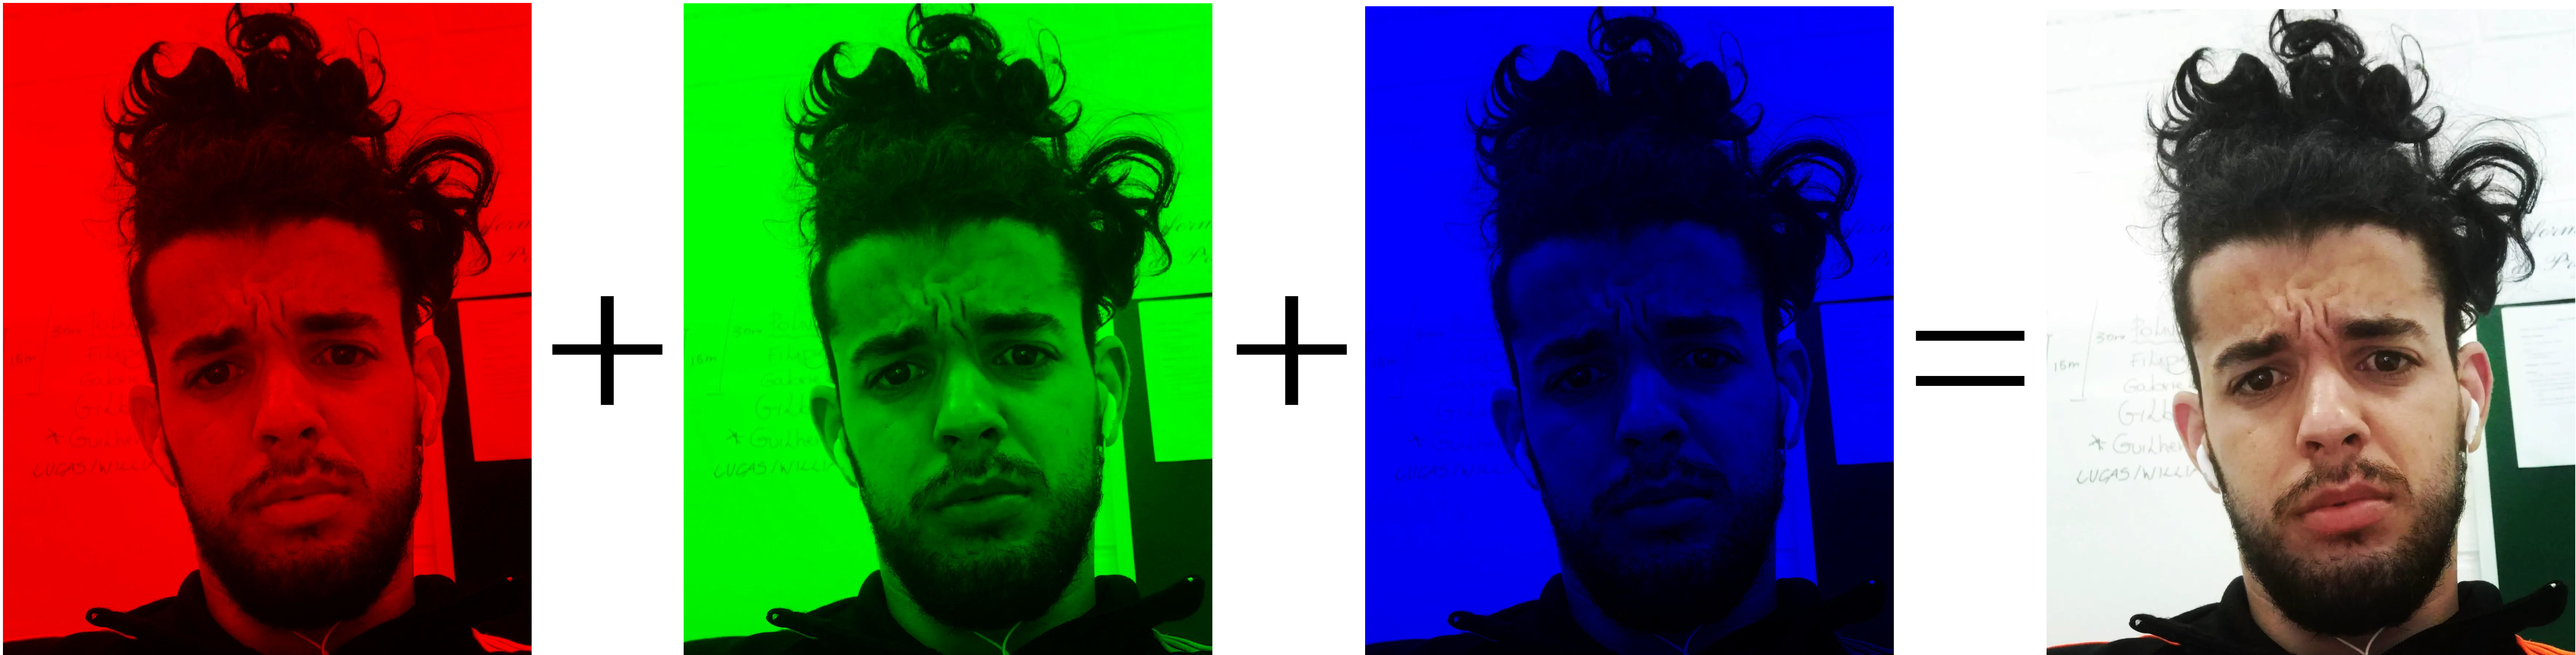
\includegraphics[scale=0.25]{figuras/Imagem_colorida/colored.png}
    \legend{Fonte: Elaborado pelo autor (2023).}
	\label{fig:Composicao de um imagem RGB}
\end{figure}

Em uma imagem digital, a descrição da intensidade da luz pode ocorrer de maneiras distintas,relacionada à natureza da imagem. A descrição da intensidade pode adotar valores binários representados por branco e preto e são frequentemente associados a conceitos como a presença ou a ausencia de um objeto.Para  uma representação mais complexa de nuances de intensidade, texturas e detalhes é comum  que a intensidade da luz seja descrita em 8 bits ou seja 256 tonalidades diferentes de cores, variando de 0 a 255, onde 0 é preto e 255 é branco.Por fim para uma riqueza maior de detalhes é comum que imagens coloridas sejam descritas por uma tripla de canais \ac{RGB}  onde cada canal representa uma  cor, adotando valores de 8 bits por canal, portanto uma representação de 24 bits por pixel\cite{imagemIBM}.

\begin{figure}[!htb]
	\centering
	\caption{Representação do Pixel de uma imagem com 3 canais}
	\includegraphics[scale=1]{figuras/processamento_imagem/pixel.png}
    \legend{Fonte:\cite{imagemIBM}.}
	\label{fig:Representacao do Pixel de uma imagem com 3 canais}
\end{figure}



\subsection[Processamento de Imagem]{Processamento de Imagem}

O processamento de imagem refere-se à manipulação de imagens digitais para obter informações relevantes ou aprimorar a qualidade da imagem original por meio da aplicação de operações específicas. Em essência, o processamento de imagem atua como um tipo de processamento de sinais, onde a entrada é uma imagem digital e a saída resulta em uma nova representação da imagem ou informações derivadas dela. O objetivo central é extrair significado ou realçar características ao empregar uma série de técnicas e algoritmos, visando melhorar a utilidade ou interpretação das imagens \cite{imagemIBM}.

O processamento de imagens abrange um conjunto de etapas interligadas, cada uma contribuindo para transformar uma imagem digital em informações compreensíveis e relevantes. Inicialmente, ocorre a "aquisição de imagens", onde os dados visuais são capturados por meio de câmeras, scanners ou sensores. Em seguida, passa-se pelo "pré-processamento", onde a imagem é preparada para análise, eliminando ruídos e melhorando o contraste. A "segmentação" divide a imagem em regiões distintas, possibilitando focar em áreas específicas. A etapa de "representação e descrição" extrai características únicas de cada região, como texturas, formas e cores. Posteriormente, o "reconhecimento e interpretação" entra em cena, empregando algoritmos para identificar padrões, objetos ou informações relevantes com base nas características extraídas anteriormente. Esse processo cíclico de aquisição, pré-processamento, segmentação, representação e descrição, bem como reconhecimento e interpretação, forma o núcleo do processamento de imagens, permitindo a compreensão e análise de informações visuais de maneira mais eficaz e detalhada\cite{imagemMonocromatica}.


\begin{figure}[!htb]
	\centering
    \caption{Fluxograma das etapas do processamento de imagens digitais}
	\includegraphics[scale=0.4]{figuras/processamento_imagem/ProcessamentoImagem.png}
    \legend{Fonte: \cite{imagemMonocromatica}.}
	\label{fig:Fluxograma das etapas do processamento de imagens digitais}
\end{figure}




\subsection[Estimativa de pose humana]{Estimativa de pose humana}\label{sec:Estimativa de pose humana}
Identificação de Pose ou \ac{EPH} é um problema geral em Visão Computacional, que tem o objetivo de detectar a posição e a orientação de uma pessoa em imagens ou vídeos prevendo a localização de alguns pontos-chaves ,conhecidos tambem como \textit{landmarks}, tais como  cabeça, ombros, cotovelos, mãos, quadril, joelhos e pés.\cite{edh}

\ac{EPH} pode ser bidimensional ou tridimensional, sendo o primeiro responsavel por estimar as cordenadas X Y e o segundo as cordenadas X Y Z de um espaço virtual que geralmente é inferido a partir de uma imagem bidimensional. A \ac{EPH} pode tambem ser classificada de acordo com a quantidade de pessoas a serem estimadas podendo ser uma unica pessoa ou de várias pessoas o que interfere nas resoluções possiveis pois a estimativa de postura de várias pessoas é ligeiramente mais difícil do que o caso de uma única pessoa.\cite{edhDeep}

\begin{figure}[!htb]
	\centering
    \caption{Captura de pontos de referência para estimativa de pose humana}
	\includegraphics[scale=0.2]{figuras/eph/keypoint.jpg}
    \legend{Fonte: \cite{tensorFlow_IMG}.}
	\label{fig:Captura de pontos de referencia para estimativa de pose humana}
\end{figure}





\subsection[Transformada de Hough]{Transformada de Hough}\label{sec:Transformada de Hough}


A Transformada de Hough é um algoritmo amplamente empregado na detecção de linhas retas em imagens. Sua utilidade é especialmente evidente ao buscar a extração de informações relacionadas a linhas presentes na imagem independentemente da orientação, localização ou contiuidade. Em suma a Transformada de Hough opera transformando coordenadas cartesianas ($x$, $y$) da imagem em uma representação polar ($\rho$, $\theta$) no espaço de parâmetros, também conhecido como plano de Hough, esse plano é usado como um espaço de votação, onde é verificado quantos pontos compartilham uma mesma reta assim as retas que acumulam mais votos no espaço de votação são consideradas as retas detectadas na imagem\cite{transformadaHough1}.


Uma reta pode ser descrita como: $$y = mx + b$$ As características desta reta são a inclinação $m$ e a intersecção $b$ assim, uma reta $y = mx + b$ pode ser representada como um par ordenado $(b, m)$, porem em tal representação à medida em que a reta torna-se vertical, as magnitudes de $b$ e $m$ tendem ao infinito, contudo a mesma reta pode ser representada na forma:  $$\rho = x*cos(\theta)+y*sin(\theta)$$ Onde o parâmetro $\rho$ é a mínima distância da reta a origem, centro do plano, e $\theta$ é o ângulo de inclinação da normal à reta, sendo a normal uma linha perpendicular a direção da reta \cite{detectBar}.

\begin{figure}[!htb]
	\centering
    \caption{Representação da reta pelos parametros $\rho$ e $\theta$}
	\includegraphics[scale=2]{figuras/math/rhotheta.png}
    \legend{Fonte: \cite{parametrizacao}.}
    \label{fig:Representacao da reta pelos parametros}
\end{figure}

O plano de Hough é um plano bidimensional onde os eixos representam os parâmetros, sendo eixo $X$ representante do ângulo $\theta$ e o eixo $Y$ a representação da distância $\rho$ \cite{transformadaHough1}. Nesse contexto, um ponto no plano da imagem é atravessado por inúmeras retas, e a combinação de todas essas retas resulta na formação de uma curva senoidal no espaço de Hough\cite{detectBar}. Na figura \ref{fig:Representacao de um ponto no espaco parametrizavel} é demonstrado um ponto no plano e logo em seguinda sua representação no espaço parametrizavel $\rho$ e $\theta$.


\begin{figure}[!htb]
	\centering
    \caption{Representação de um ponto no espaço parametrizavel $\rho$ e $\theta$}
	\includegraphics[scale=0.5]{figuras/math/pontoEspacoParametrizavel.png}
    \legend{Fonte: \cite{parametrizacao}.}
	\label{fig:Representacao de um ponto no espaco parametrizavel}
\end{figure}

Dois pontos $p$ e $q$ no plano da imagem definem uma reta $pq$ e correspondem a dois senóides no plano de Hough, a intersecção dos dois senóides representa a reta $pq$ que
passa pelos dois pontos no plano da imagem, analogamente 4 retas no plano da imagem correspondem a 4 senóides no plano de Hough que se acumulam em 4 pontos, portanto, para realizar a detecção de uma reta, é necessário examinar as interseções das curvas senoidais. Isso é alcançado por meio da utilização de um acumulador, que consiste em uma lista destinada a armazenar todos os cruzamentos identificados. O processo de detecção de retas, consiste em selecionar os cruzamentos que apresentam maior frequência na lista do acumulador \cite{transformadaHough2}. Na figura \ref{fig:Representacao da reta por meio do ponto de interseccao} é demonstrado 8 pontos no plano pertencentes a 2 retas e logo em seguinda sua representação no espaço parametrizavel $\rho$ e $\theta$ que se da por meio da intersecção das curvas, sendo assim o local da interseção das 4 curvas representam uma reta com parametros $\rho$ e $\theta$ específicos.

\begin{figure}[!htb]
	\centering
    \caption{Representação da reta por meio do ponto de intersecção}
	\includegraphics[scale=0.5]{figuras/math/senoidesIterseccao.png}
    \legend{Fonte: \cite{parametrizacao}.}
	\label{fig:Representacao da reta por meio do ponto de interseccao}
\end{figure}





\subsection[Detector de bordas de Canny]{Detector de bordas de Canny}\label{sec:Detector de bordas de Canny}

Um filtro de detecção de borda é um método utilizado no processamento de imagens para identificar mudanças abruptas na intensidade luminosa. Essas mudanças geralmente correspondem a limites entre diferentes objetos ou regiões na imagem. O filtro de detecção de borda realça essas mudanças, destacando os contornos e limites dos objetos presentes na imagem. Ele funciona calculando gradientes de intensidade em várias direções e destacando as regiões onde esses gradientes são mais acentuados. Em específico o filtro de Canny possui cinco etápas sendo elas: Redução de ruído; Cálculo de gradiente; Supressão não máxima; Limite duplo;Rastreamento de borda por histerese\cite{canny-edge-detection-python}.


\subsubsection[Redução de ruido]{Redução de ruido}
A redução de ruido ocorre com a aplicação de um filtro Gaussiano, uma técnica de convolução de imagens que de acordo com um filtro substitue o valor de cada pixel da imagem pela média da vizinhança, tendo como efeito a suavização da imagem, uma vez que as altas frequências que correspondem às transições abruptas são atenuadas\cite{filtroGaus}.

A convolução é uma operação matemática que combina duas funções para criar uma terceira. No contexto de processamento de imagens, a imagem original atua como uma das funções e o filtro (ou kernel) atua como a segunda função. O filtro é uma matriz de números que define como a vizinhança de cada pixel na imagem será ponderada e combinada para gerar o novo valor desse pixel na imagem resultante. O processo de convolução envolve a superposição do filtro sobre cada região da imagem e a multiplicação elemento a elemento dos valores do filtro com os valores correspondentes da imagem. Os resultados dessas multiplicações são somados para produzir o novo valor do pixel na imagem de saída\cite{convolucao}.

Kernel 5x5 utilizado no filtro gaussiano \cite{kernel_gaus}:

\[
    \begin{bmatrix}
        1 & 4 & 7 & 4 & 1 \\
        4 & 16 & 26 & 16 & 4 \\
        7 & 26 & 41 & 26 & 7 \\
        4 & 16 & 26 & 16 & 4 \\
        1 & 4 & 7 & 4 & 1 \\
    \end{bmatrix}
\]

O tamanho do kernel esta relacionado com o efeito de desfoque, quanto menor o kernel, menos visível é o desfoque, no filtro de canny é usado um kernel 5x5.





\subsubsection[Calculo do Gradiente]{Calculo do Gradiente}

As bordas correspondem a uma mudança na intensidade dos pixels portanto o calculo do gradiente em processamento de imagem refere-se à taxa de variação da intensidade luminosa em uma determinada região da imagem essa variação pode ser calculada usando operadores de detecção de borda na horizontal e vertical, ou seja convolucionando a imagem com os respectivos kernels:

Filtro Sobel Horizontal:
\[
    \begin{bmatrix}
        -1 & 0 & 1 \\
        -2 & 0 & 2 \\
        -1 & 0 & 1 \\
    \end{bmatrix}
\]

Filtro Sobel Vertical:
\[
    \begin{bmatrix}
        1 & 2 & 1 \\
        0 & 0 & 0 \\
        -1 & -2 & -1 \\
    \end{bmatrix}
\]


Aplicando o filtro de sobel na horizontal tem se $G_x$ que é o gradiente na direção horizontal e aplicando o filtro de sobel na vertical tem se $G_y$ que é gradiente na direção vertical, fazendo uso dessas informações é possivel chegar a  $G_r$ com a formula:

$$G_R = \sqrt{G_x^2 + G_y^2}$$

$G_r$ se refere ao valor resultante da combinação dos gradientes em duas direções (horizontal e vertical) pontos onde $G_r$ é alto indicam mudanças bruscas de intensidade, muitas vezes correspondendo a bordas ou detalhes significativos na imagem. 

A inclinação $\theta$ que informa a direção do gradiente é calculado pela formula:
$$\theta(x,y) = \tan^{-1}\left(\frac{G_y}{G_x}\right)$$

Essa inclinação é perpendicular às arestas e arredondado para um dos quatro ângulos que representam as direções vertical, horizontal e duas diagonais.



\begin{figure}[!htb]
	\centering
    \caption{Imagem em preto e branco com filtro gaussiano}
	\includegraphics[scale=0.25]{figuras/filter/sobel/f_normal.jpeg}
    \legend{Fonte: Elaborado pelo autor (2023)}
	\label{fig:Imagem em preto e branco com filtro de gaus}
\end{figure}

\begin{figure}[!htb]
	\centering
    \caption{Intensidade da mudança de gradiente usando operador de Sobel}
	\includegraphics[scale=0.25]{figuras/filter/sobel/f_sobel.jpeg}
    \legend{Fonte: Elaborado pelo autor (2023)}
	\label{fig:Intensidade da mudanca de gradiente}
\end{figure}



\subsubsection[Supressão não máxima]{Supressão não máxima}


É desejável que a imagem resultante apresente bordas precisas e nítidas, para alcançar esse objetivo, aplicasse uma supressão não-máxima, a fim de refinar as bordas detectadas. Nesse processo, o algoritmo percorre todos os pontos da matriz de intensidade de gradiente, nos locais onde as bordas são encontradas, o algoritmo  assegura que o pixel que é um máximo local dentro de sua vizinhança na orientação do gradiente seja mantido e os que não são, sejam suprimidos\cite{canny-edge-detection-python}.



\begin{figure}[!ht]
	\centering
    \caption{Supressao não maxima}
	\includegraphics[scale=0.65]{figuras/filter/supressao_nao_maxima/supressao3.png}
    \legend{Fonte: \cite{canny-edge-detection-python}.}
	\label{fig:Supressao nao maxima}
\end{figure}


O procedimento do algoritmo é ilustrado na figura \ref{fig:Supressao nao maxima} onde: o pixel que está destacado em vermelho é aquele que está sendo processado. A linha em laranja representa a orientação do gradiente ou seja é uma linha perpendicular à borda, os pixels de interesse presentes na vizinhança são aqueles que estão destacados em azul, uma vez que estão na mesma orientação do gradiente. Se o valor do pixel realçado em vermelho for maior do que o valor dos pixels vizinhos destacados em azul, então esse pixel será mantido. Caso contrário, ele será suprimido, assegurando que somente os pontos mais significativos sejam preservados na representação das bordas\cite{canny-edge-detection-python}.




\subsubsection[Limite duplo]{Limite duplo}

O "limiar duplo" é uma técnica usada no processamento de imagens para segmentar uma imagem com base nos valores de intensidade dos pixels. Essa técnica envolve a definição de dois limiares diferentes, um limiar inferior $minVal$ e um limiar superior $maxVal$. Esses limiares dividem a escala de intensidade dos pixels em três intervalos: pixels abaixo de $minVal$, pixels entre $minVal$ e $maxVal$ e pixels acima de $maxVal$.

Com base nos limiares definidos, os pixels são definidos em três tipos:
Pixels abaixo de $minVal$ são desconsiderados pois não possuem uma itensidade minima para ser considerado relevante.
Pixels entre $minVal$ e  $maxVal$ são atribuídos à região de transição no qual é necessário uma outra análise.
Pixels acima de  $maxVal$ são atribuídos à região de interesse pois certamente contribuem para a borda final.\cite{canny-edge-detection-python}


\subsubsection[Limite de histerese]{Limite de histerese}

Baseado no limite duplo, o limite de histerese atua sobre os pixels que estão entre $minVal$ e $maxVal$,  transformando pixels possivelmente relevante em certamente relevantes se e somente se pelo menos um dos pixels ao redor daquele que está sendo processado for relevante, conforme descrito abaixo:


Os pixels que estão entre $minVal$ e  $maxVal$  são classificados como bordas ou não-bordas com base em sua conectividade. Se eles estiverem conectados a pixels  superiores a  $maxVal$, eles serão considerados parte das bordas, caso contrário serão descartados. Além das vizinhanças imediatas, verificações recursivas ou iterativas podem ser realizadas para explorar os pixels vizinhos dos pixels já marcados como relevantes. Isso permite estender a borda para pixels que não são diretamente vizinhos, mas que são alcançáveis por meio de pixels relevantes interligados.\cite{opencv-canny}






\subsection[Algoritmo de rastreamento ou Tracking]{Algoritmo de rastreamento ou Tracking}

O rastreamento, também conhecido como \textit{tracking}, pode ser conceituado como um conjunto de procedimentos computacionais elaborados com o propósito de monitorar e seguir o movimento ou a posição de objetos em uma sequência de imagens ao longo do tempo. Um algoritmo de rastreamento eficiente utiliza informações acumuladas sobre o objeto até o momento baseado no modelo de movimento do objeto que engloba  sua posição, sua velocidade e direção do movimento e baseado tambem no modelo de aparência, que proporciona informações sobre a aparência específica do objeto baseada nos quadros anteriores, ou seja,  enquanto a detecção de objetos ocorre em quadros de imagem isolados, o algoritmo de rastreamento é aplicado com base em uma sequência temporal, permitindo uma análise contínua do movimento do objeto\cite{tracking}.

O modelo de aparência desempenha um papel crucial no processo, permitindo a realização de uma busca precisa em uma pequena área próxima à localização prevista pelo modelo de movimento o que  otimiza o processo de rastreamento, pois ocorre uma pesquisa local em vez de uma pesquisa global garantindo a identidade do objeto,sendo assim mesmo com uma oclusão do objeto é possível rastrear o objeto, porque o rastreamento leva em consideração a localização e a aparência do objeto no quadro anterior. Entretanto, esse processo pode enfrentar desafios consideráveis, como a perda do objeto quando ele fica obstruído por um período prolongado ou quando sua velocidade é tão elevada que o algoritmo de rastreamento não consegue acompanhá-lo, por isso é comum que os algoritmos de rastreamento acumulem erros ao longo do tempo, comprometendo a precisão da localização do objeto. Para mitigar essas questões inerentes aos algoritmos de rastreamento, uma abordagem utilizada é executar periodicamente um algoritmo de detecção para identificação da nova posição do objeto e, em seguida retransmitir essas informações para o rastreador, afim de contribuir para a correção dos erros acumulados e manter um acompanhamento mais preciso do objeto ao longo do tempo\cite{tracking}.


Diversos algoritmos de rastreamento de objetos podem ser identificados, cada um com suas características particulares. Alguns exemplos notáveis incluem a Subtração de Plano de Fundo, o Casamento de Blocos, o \ac{SIFT}, e o \ac{RANSAC}.

A Subtração de Plano de Fundo é capaz de identificar objetos destacando discrepâncias entre o plano de fundo e os objetos em movimento na cena. Por sua vez, o Casamento de Blocos realiza a comparação de blocos de pixels em diferentes quadros, o que lhe permite rastrear o movimento de objetos com eficácia. O algoritmo \ac{SIFT} desempenha um papel crucial ao extrair características distintivas de uma imagem, possibilitando o rastreamento robusto de objetos, mesmo diante de variações na escala, rotação ou iluminação. Finalmente, o \ac{RANSAC} é empregado para a estimativa de parâmetros de um modelo matemático previamente definido, de forma a se ajustar ao maior número possível de dados, ou seja, aqueles que são comumente chamados de "inliers". Esses algoritmos oferecem soluções diversas e adaptáveis para a tarefa de rastreamento de objetos, cada um adequado a diferentes cenários e requisitos de aplicação \cite{tracking-algoritimo}.











\subsection[Pixelização]{Pixelização}

Quando uma imagem é ampliada ou exibida em uma resolução maior do que sua resolução original, os pixels individuais se tornam visíveis, resultando em uma aparência granulada ou \aspas{pixelizada} pois os detalhes da imagem original não podem ser representados com precisão em uma resolução mais baixa. Portanto o filtro de pixelização se resume em reduzir o número de valores de pixel distintos em uma imagem substituindo um bloco quadrado de valores de pixel por seu valor médio\cite{pixelizacao}




\begin{figure}[htbp]
    \centering
    \caption{Imagem pixelizada com blocos de 32x32}
        \begin{minipage}{0.4\textwidth}
            \includegraphics[width=\textwidth]{figuras/pixelizacao/foto.jpeg}
        \end{minipage}
        \begin{minipage}{0.4\textwidth}
            \includegraphics[width=\textwidth]{figuras/pixelizacao/32.png}
        \end{minipage}
    \legend{Fonte: Elaborado pelo autor (2023)}
    \label{fig:Imagem pixelizada}
\end{figure}











\subsection[Limiarização]{Limiarização}

A limiarização, também conhecida como \textit{thresholding}, é uma técnica de processamento de imagem usada para classificar os pixels em uma imagem com base em um valor específico, denominado limiar. Isso resulta na categorização dos pixels em dois grupos distintos, geralmente sendo aqueles que têm valores acima do limiar e aqueles que têm valores abaixo ou iguais a ele. Esse método é amplamente utilizado em processamento de imagem para destacar ou segmentar objetos de interesse em relação ao restante da imagem \cite{limiarizacao}.

A limiarização pode ser empregada de duas maneiras distintas: ela pode transformar uma imagem em escala de cinza em uma imagem binarizada, tornando os pixels acima do limiar em branco e os pixels abaixo do limiar em preto. Alternativamente, ela pode ser utilizada para enfatizar uma faixa específica de frequência, convertendo apenas os pixels abaixo do limiar em preto ou apenas os pixels acima do limiar em branco\cite{opencv_thresholding}.


\section[Machine learning]{Machine learning}\label{sec:Machine learning}

Aprendizado de Máquina tambem conhecido como \ac{ML} é um ramo da \ac{IA} focado na análise de dados, que por meio de métodos estatísticos de aprendizado e otimização  permite computadores analisarem conjuntos de dados e identificar padrões e tendências históricas para prever modelos futuros.\cite{ml}

Comumente o algoritmo de aprendizado de máquina supervisionado consiste em três componentes: decisão, erro e otimização. 

O primeiro componente, decisão, é responsável por tomar decisões com base nas entradas fornecidas, que podem ser rotuladas ou não rotuladas. Esse componente é geralmente implementado como uma função matemática que mapeia as entradas para uma saída, seja uma classificação ou uma predição. Ele é responsável por transformar as entradas em informações úteis para o modelo, permitindo que o algoritmo aprenda a partir delas e tome decisões com base em novas entradas no futuro.

O segundo componente, erro, é responsável por avaliar a precisão da classificação ou da saída predita em relação à saída verdadeira, ou seja, os exemplos conhecidos. Esse componente é crucial porque permite uma analise do modelo.


O terceiro componente, otimização, é responsável por ajustar o modelo de modo que  minimize o  erro calculado pelo segundo componente e consequentemente seja possivel melhorar a precisão da saída predita. 



\section[Automatos Finitos]{Automatos Finitios}


Os reconhecedores são sistemas formais conhecidos tambem como autômatos capazes de aceitar todas as sentenças que pertençam a uma determinada linguagem, rejeitando todas as demais. Por esse motivo, constituem uma forma alternativa às gramáticas para a representação finita de linguagens.\cite{reconhecimento}

Os reconhecedores apresentam quatro componentes fundamentais: uma memória (fita) contendo o texto de entrada do
reconhecedor, um cursor, que indica o próximo elemento da fita a ser processado, uma máquina de estados finitos, sem memória, e uma memória auxiliar opcional.


\begin{figure}[!htb]
	\centering
    \caption{Organização de um reconhecedor genérico}
	\includegraphics[scale=2]{figuras/AFD/reconhecedor.png}
    \legend{Fonte: \cite{AFD_reconhecedor}.}
	\label{fig:Organizacao de um reconhecedor generico}
\end{figure}


A fita de entrada é composta pela cadeia que o reconhecedor precisa analisar. Ela é dividida em células, cada uma contendo um único símbolo da sequência, que faz parte do alfabeto de entrada escolhido. A sequência é organizada da esquerda para a direita, começando pelo símbolo mais à esquerda na fita. O cursor, chamado normalmente de cabeçote de acesso, é utilizado para ler os símbolos da fita de entrada. Ele aponta sempre para o próximo símbolo que deve ser processado. Os movimentos do cursor são controlados pela máquina de estados, podendo ser unidirecionais (em geral, movendo-se apenas para a direita) ou bidirecionais (movendo-se tanto para a esquerda quanto para a direita), dependendo do tipo de reconhecedor\cite{reconhecimento}.

Alguns tipos de reconhecedores não apenas leem os símbolos da fita de entrada, mas também escrevem sobre a fita, substituindo os símbolos existentes por outros, de acordo com comandos definidos pela máquina de estados. A máquina de estados atua como o cérebro do reconhecedor, contendo um conjunto finito de estados que registram as informações coletadas e guiam o funcionamento do processo\cite{reconhecimento}.


Um \ac{AF} é um modelo abstrato e simplificado de um sistema computacional que pode ser usado para reconhecer padrões em sequências de símbolos \cite{afd}. Formalmente é representado como uma lista de cinco elementos  com : 
um conjunto finito de estados representado por $Q$, um alfabeto de entrada representado por $\Sigma$, Funções de transição representada por $\delta : Q \times \Sigma \rightarrow Q$, estado inicial $q_0 \in Q$ e um conjunto de estados finais $F \subseteq Q$ portanto um automato finito é representado como uma 5-upla $(Q, \Sigma, \delta, q_0, F)$

Sendo que o estado é uma representação de uma condição específica em que o autômato pode se encontrar durante a sua execução, o alfabeto é o conjunto finito de símbolos que o autômato pode receber como entrada, e as funções de transição definem como o autômato muda de um estado para outro em resposta a um símbolo de entrada.

As funções de transição são denotadas como $\delta(e_0, 1) = e_1$, em outras palavras, essa regra específica indica que um autômato no estado $e_0$, ao ler o caractere 1, se move para o estado $e_1$.

Tambem é possivel representar um \ac{AF} de modo mais visual por meio de um diagrama de estados onde é ilustrado os estados do autômato, suas transições e os símbolos de entrada. Cada estado é representado por um círculo e as transições são indicadas por setas entre esses círculos, rotuladas com os símbolos de entrada correspondentes.\cite{afd}

Em um diagrama de estados, cada estado é representado por um círculo, enquanto as transições são marcadas por setas que conectam esses círculos. Essas setas são rotuladas com os símbolos de entrada correpondentes. O estado inicial é indicado com uma seta apontando para ele, originada de um ponto vazio. Os estados de aceitação são ilustrados por círculos duplos.

Portanto um \ac{AF} chamado $M_1$ que aceita qualquer numero binário impar pode ser representado de 2 maneiras,  por uma 5-upla ou um diagrama de estados:

\begin{itemize}
    \item[$M_1$] = $(Q, \Sigma, \delta, q_1, F)$, onde:
    \item[$Q$] = $\{q_1, q_2, q_3\}$
    \item[$\Sigma$] = \{0,1\}
    \item [$\delta$] é descrito como
    \item [ ]
        \begin{tabular}{c|cc}
            & 0 & 1 \\ \hline
            $q_1$ & $q_1$ & $q_2$ \\
            $q_2$ & $q_3$ & $q_2$ \\
            $q_3$ & $q_2$ & $q_2$ \\
        \end{tabular}
    \item[$q_1$] é o estado inicial
    \item[$F$] = \{$q_2$\}
\end{itemize}

\begin{figure}[!htb]
	\centering
    \caption{Diagrama de estados de $M_1$}
	\includegraphics[scale=1]{figuras/AFD/m1.png}
    \legend{Fonte: \cite{AFD_M1}.}
	\label{fig:Diagrama de estados}
\end{figure}

Um reconhecedor e um \ac{AF} são conceitos relacionados, mas cada um tem um papel específico sendo esse um modelo abstrato e aquele um sistema ou algoritmo que é capaz de identificar ou detectar algo em um conjunto de dados.





